\chapter{人和物体交互的域内泛化}\label{chap:stackflow_plus}
开放场景中的物体形状具有较高多样性,学习如何跟未曾见过物体交互对算法能否应用到自然场景中至关重要,前置章节所提出的算法从数据集中学习实例级别的交互先验,并在测试时只能将从训练集学习到的先验应用到相同的物体中,对于未曾见过的物体泛化能力较差。为了克服该泛化能力弱的缺陷,本章提出基于种类级别的交互先验学习算法,该算法构建出物体形状归一化映射,将物体映射到统一的形状空间中,在该形状空间中建立人和物体之间的交互关系。在CHAIRS数据集上的实验表明,该算法对同类别的未曾见过的物体仍然保持很强的泛化能力。

\section{人-物交互关系的先验空间构建}

给定物体$O = (\hat{\mathbf{V}}^{\text{o}}, \mathbf{E}^{\text{o}})$,章节\ref{sec:offset-representation}提出基于偏移量的编码方式来刻画人与该物体交互时的三维空间关系,对每一个以$\{\mathbf{\beta}, \mathbf{\theta}, \mathbf{R}, \mathbf{t}\}$为参数人-物交互实例,计算锚点之间的偏移量,并利用特征值分解的方式将偏移量映射到隐式空间中,得到基于偏移量的表征$\mathbf{\gamma}$,即
\begin{equation}
	\mathbf{\gamma} = R_{O} (\mathbf{\beta}, \mathbf{\theta}, \mathbf{R}, \mathbf{t}),
\end{equation}
式中,$R_{O}$是物体$O$的空间关系编码函数,该种基于人-物锚点偏移量的编码方式建立在物体$O$的拓扑结构已知的前提下,对于未曾见过的其它形状的物体失效。为了解决对其它物体泛化能力差的问题,本节提出使用物体形状映射函数$D$将物体归一化到和交互相关联的形状空间$\mathcal{O}$中,在该空间中,物体的形状被归一化,其拓扑结构只被保留和人交互中最相关的部位。而后将人和物体空间关系的编码函数$R_{\mathcal{O}}$建立在该形状空间之上,即使对于未曾见过的物体$O'$,在经过形状映射函数$D$之后得到了对物体形状的统一化表达,而人和物体间交互编码建立在$\mathcal{O}$之上,因而对于未见过的$O'$也保持强泛化能力。

\subsection{物体归一化映射函数}
人总是和物体特定的位置交互,同类物体的形状虽千奇百怪,但其内在却存在相似的拓扑结构和统一的可交互部位,为提取物体中和交互相关联的部位,使用物体形状归一化映射函数$D$,该函数将物体形状映射到与交互相关联的形状空间$\mathcal{O}$中。

如图\ref{fig:learn-object-inter-shape}所示,给定物体$O=(\hat{\mathbf{V}}^\text{o}, \mathbf{E}^{\text{o}})$,使用体素编码器$E$提取物体的形状特征$\mathbf{c}$,
\begin{equation}
	\mathbf{c} = E(\mathbf{O}),
\end{equation}
式中,$\mathbf{O}\in \mathbb{R}^{N\times N \times N}$是从物体$O$中提取的体素网格(voxel grid),$N\in \mathbb{N}$为该体素的分辨率,体素编码器$E$是由多层3D卷积网络构成,最后使用池化层对体素特征降采样得到物体的形状编码$\mathbf{c}$。形状映射函数$D$是由一组级联的网格模型形变器组成,该网格模型形变器从初始椭球体$\mathcal{S}=(\hat{\mathbf{S}}^{(0)}, \mathbf{E}^{\mathcal{S}})$出发,逐步对椭球体初始顶点$\hat{\mathbf{S}}^{(0)}$添加偏置,最终得到物体目标形状$D(\mathbf{O})=(\hat{\mathbf{S}}^{\star}, \mathbf{E}^{\mathcal{S}})$。每一层网格模型形变器由基于残差连接的图卷积层构成,以上一层的顶点作为输入,产生下一层的顶点,即
\begin{equation}
	\hat{\mathbf{S}}^{(i+1)} = \text{G-ResNet}(\hat{\mathbf{S}}^{(i)} \oplus \mathbf{c}, \mathbf{E}^{\mathcal{S}}),
\end{equation}
式中,G-ResNet为基于残差连接的图卷积网络\citep{Pixel2Mesh},$\oplus$表示特征按照维度相连接,$\mathbf{c}$是从物体$O$提取的特征,$\mathbf{E}^{\mathcal{S}}$为初始椭球体的边。归一化后的物体网格模型$D(\mathbf{O})=(\hat{\mathbf{S}}^\star, \mathbf{E}^{\mathcal{S}})$共享一组边集,并且具有相同数量的顶点。

\begin{figure}[!htbp]
	\centering
	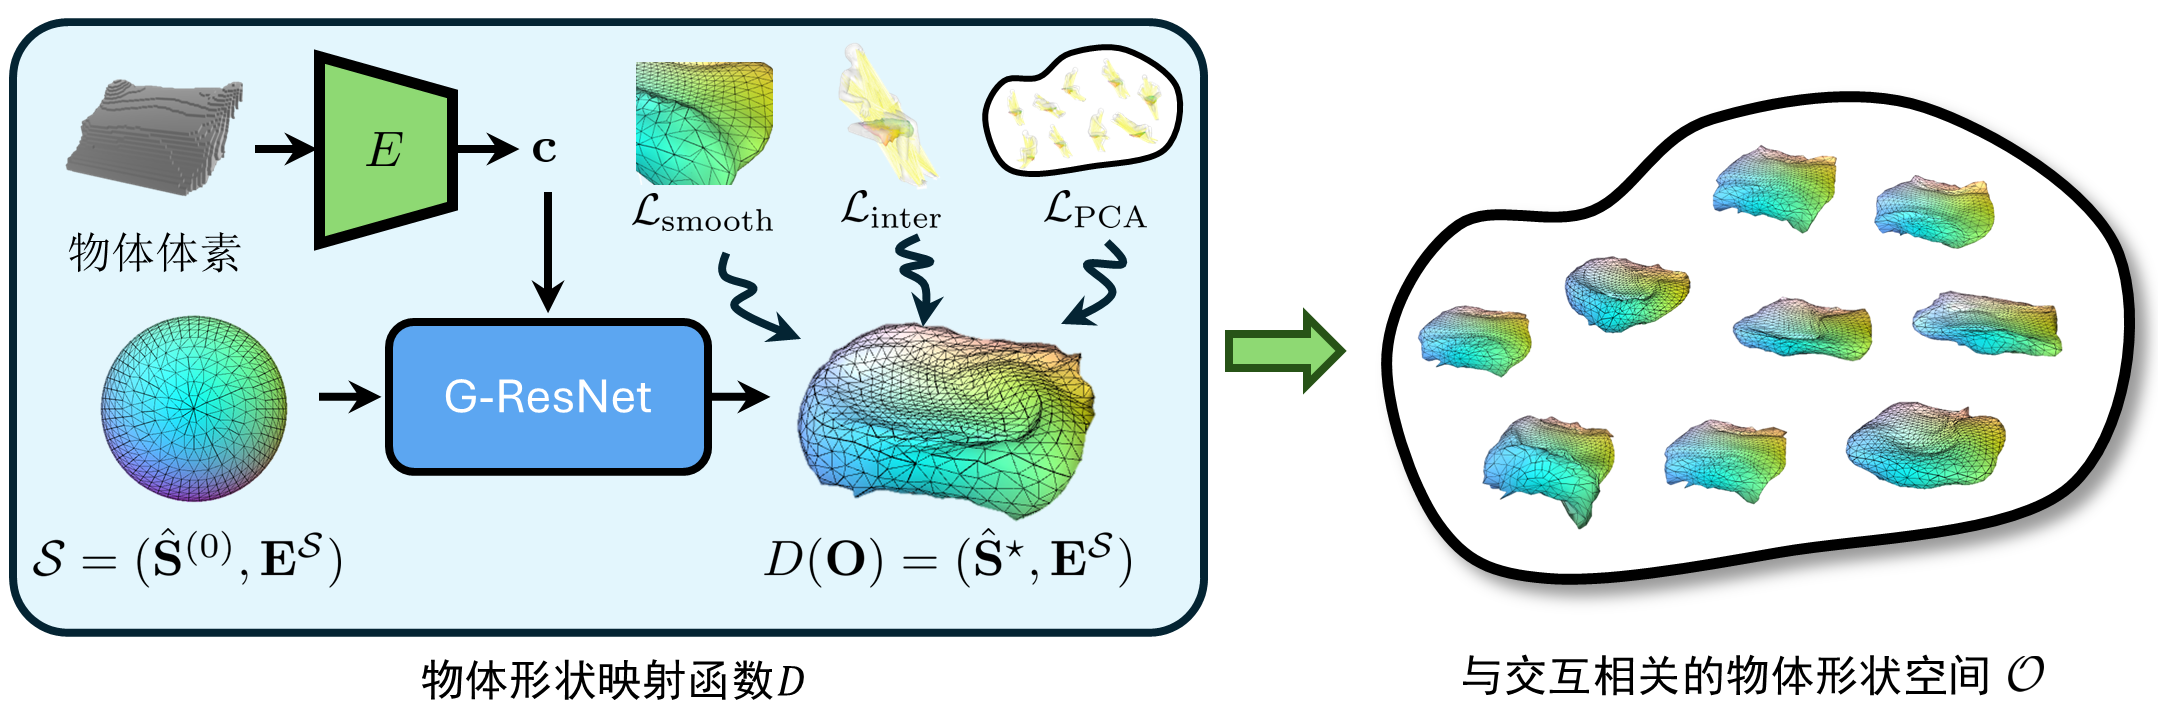
\includegraphics{Img/learn_object_shape}
	\bicaption{学习物体形状归一化映射流程图。}{The pipeline of the procedure of learning interaction-relatied shape mapping.}
	\label{fig:learn-object-inter-shape}
\end{figure}

\subsection{人物关系编码}
在章节\ref{sec:offset-representation}提出的编码方式中,物体锚点采样于特定形状物体的网格模型表面,使用该锚点对应的偏移量所构建的隐式空间只能作用于该物体,不能泛化到其他形状的物体,而本章所提出的编码方式中,物体的锚点采样于初始椭球体$\mathcal{S}$,所有物体经过归一化映射之后,网格模型顶点数量相同且具有相同的拓扑连接结构,因而锚点索引集合可以被所有物体共享。从物体的初始椭球体$\mathcal{S}$表面均匀随机选取$n$个点,记录该$n$个点的索引形成物体的锚点索引集合$\mathcal{A}_{\mathcal{O}}$,对于每一个物体$O$,其锚点取自于形状归一化后的物体模型$D(\mathbf{O})$,人体锚点的选取方式和章节\ref{sec:offset-representation}保持一致。偏移量计算方式由式(\ref{eq:offset})改成
\begin{equation}
	\mathbf{d}_{i,j} = \mathbf{S}^{\star}_j - \mathbf{V}_i^{\text{h}}, i \in \mathcal{A}_{\text{h}}, j \in \mathcal{A}_{\mathcal{O}},
\end{equation}
式中,$\mathbf{S}^\star_j = \mathbf{R} \hat{\mathbf{S}}^\star_j + \mathbf{t}$为物体归一化后的顶点在SMPL模型局部坐标系下的坐标。在该种计算方式下,人-物交互实例对应的空间关系编码会随着物体映射函数$D$的变化而变化,使用增量式主成分分析\citep{Ross2008IncrementalLF}来自适应学习人物空间关系编码,该增量式学习的过程伴随物体映射函数$D$学习的过程,增量式主成分分析逐步从数据中学习空间投影矩阵$\mathbf{P}$和数据均值$\mathbf{\mu}$。在增量式学习空间关系编码过程中,对于每一批次的偏移量$\mathbf{X}_{\text{batch}} \in \mathbb{R}^{p \times 3mn}$,计算矩阵$[f\mathbf{\Sigma} \mathbf{P}^T,\\ \mathbf{X}_{\text{batch}} - \bar{\mathbf{X}}_{\text{batch}}, \sqrt{\frac{pq}{p + q}}(\bar{\mathbf{X}}_{\text{batch}} - \mathbf{\mu})]$的奇异值分解,即
\begin{equation}
	\hat{\mathbf{U}}\hat{\mathbf{\Sigma}}\hat{\mathbf{V}}^T = \text{SVD}([f\Sigma \mathbf{P}^T, \mathbf{X}_{\text{batch}} - \bar{\mathbf{X}}_{\text{batch}}, \sqrt{\frac{pq}{p + q}}(\bar{\mathbf{X}}_{\text{batch}} - \mathbf{\mu})]),
\end{equation}
式中,$\bar{\mathbf{X}}_{\text{batch}}$表示当前批次偏移量的均值,$p$为当前批次样本个数,$q$表示截至目前所迭代过样本的总数,$f$是遗忘因子,$\mathbf{\Sigma}$为投影矩阵$\hat{\mathbf{P}}$中各个维度的方差,经奇异值分解后,取$\hat{\mathbf{\Sigma}}$前$k$个较大的方差和$\mathbf{V}$中对应的向量来更新$\mathbf{\Sigma}$和$\mathbf{\mathbf{P}}$,均值向量$\mathbf{\mu}$按照下式更新,
\begin{equation}
	\mathbf{\mu} \gets \frac{p}{p + fq} \bar{\mathbf{X}}_{\text{batch}} + \frac{fq}{p + fq}\mathbf{\mu}.
\end{equation}

投影矩阵$\mathbf{P}$和数据的均值$\mathbf{\mu}$伴随着物体映射函数的学习,在物体映射函数的学习过程中,人和物体之间的偏移量会随着被映射后的物体的形状而逐步变化,$\mathbf{P}$和$\mathbf{\mu}$会伴随物体的形状而逐步更新。

\subsection{训练}
训练该形状映射函数$D$的损失函数包含网格模型平滑损失、人物交互损失和特征分解损失。为了提取物体和人体交互最相关的区域,对人和物体频繁交互的区域做出损失,使得物体在映射后形状能够保持其可交互的特性。记$d(\mathbf{v}, \mathbf{V})$为点$\mathbf{v}$到点集$\mathbf{V}$的最短距离,与人相交互的损失为
\begin{equation}
	\mathcal{L}_{\text{inter}} = \sum_{\mathbf{v} \in \mathbf{V}^{\text{h}}} w(\mathbf{v}) \cdot \| d(\mathbf{v}, \mathbf{V}^{\text{o}}) - d(\mathbf{v}, \mathbf{S}^{\star}) \|_1,
\end{equation}
式中,$w(\mathbf{v})$的在点$\mathbf{v}$处的权重,其计算方式为
\begin{equation}\label{eq:weighting}
	w(\mathbf{v}) = f(d(\mathbf{v}, \mathbf{V}^\text{o})) + f(d(\mathbf{v}, \mathbf{S}^\star)) - f(d(\mathbf{v}, \mathbf{V}^\text{o})) \cdot f(d(\mathbf{v}, \mathbf{S}^\star)),
\end{equation}
式中$f(x) = (\alpha x + 1) \cdot e^{- \alpha x}$为权重函数,$\alpha$为大于0的常数,当$x\to 0^+$,$f(x) \to 1$,当$x\to +\infty$,$f(x)\to0$。式(\ref{eq:weighting})计算权重的方式很好的平衡了那些和交互关联度高的点和外围点,当点$\mathbf{v}$处于交互区域,即该点距离物体网格模型较近,$f(\mathbf{v}, \mathbf{V}^{\text{o}}) \simeq 1$,$w(\mathbf{v}) \simeq 1$,此时损失促使$\mathbf{S}^\star$和目标物体$\mathbf{V}^\text{o}$的对应部分相匹配,相反如果点$\mathbf{v}$处于非交互区域,此时点$\mathbf{v}$周围应该处于空区域,$f(d(\mathbf{v}, \mathbf{V}^\text{o})) \simeq 0, w(\mathbf{v}) \simeq f(d(\mathbf{v}, \mathbf{S}^\star))$,损失会促使$\mathbf{S}^\star$远离该点以防发生穿模。

为了使重建后的模型能够保持平滑,使用平滑损失
\begin{equation}
	\mathcal{L}_\text{smooth} = \mathcal{L}_{\text{edge}} + \mathcal{L}_{\text{mesh}},
\end{equation}
式中,$\mathcal{L}_{\text{edge}} = \sum_{(u, v) \in \mathbf{E}^{\mathcal{S}}} \| \mathbf{S}^\star_u - \mathbf{S}_v^\star \|$,$\mathcal{L}_{\text{mesh}}$为网格模型的拉普拉斯平滑损失,其具体形式参照\citep{Nealen2006LaplacianMO}。

章节\ref{sec:offset-representation}为了构建隐式空间使用离线主成分分析,该离线主成分分析是构建在物体形状已知的前提下。而在本章中,物体形状是由映射函数$D$得到的,为此使用增量式主成分分析\citep{Ross2008IncrementalLF}学习投影矩阵$\mathbf{P}$和均值向量$\mathbf{\mu}$。在增量式主成分分析中,$\mathbf{P}$和$\mathbf{\mu}$随物体映射函数的改变而改变,为了使物体映射函数能够重构出和交互相关的形状,并且约束隐式空间,最小化投影函数$\mathbf{P}$的核范数,即
\begin{equation}
	\mathcal{L}_{\text{PCA}} = \| \mathbf{P} \|_*.
\end{equation}
因此,在训练物体形状映射函数和构建隐式空间阶段时的损失为
\begin{equation}
	\mathcal{L} = \lambda_{\text{inter}} \mathcal{L}_{\text{inter}} + \lambda_{\text{smooth}} \mathcal{L}_{\text{smooth}} + \lambda_{\text{PCA}} \mathcal{L}_{\text{PCA}}.
\end{equation}
在实验中,$\lambda_{\text{inter}} = \lambda_{\text{smooth}} = 1, \lambda_{\text{PCA}} = 1e-4$。

\section{重建算法}
将学习得到的物体形状归一化映射函数和基于偏移量的人-物空间编码应用到人-物重建任务中,为建立图片和人-物空间关系的映射,采用章节\ref{sec:stackflow}提出的叠层归一化流结构。使用预先训练好的物体形状归一化映射函数将物体的形状映射到形状空间$\mathcal{O}$,并使用主成分分析提取人-物空间关系的特征$\mathbf{\gamma}$,使用提取的特征训练归一化流模型,使其从数据集中学习概率密度$p_{\Gamma|\mathcal{I}}(\mathbf{\gamma}|\mathbf{c})$,训练归一化流模型时,物体形状归一化映射函数和人-物空间编码保持不变。在预测过程中,使用该归一化流模型从给定的图片中建立人-物空间关系的概率密度,并按照式(\ref{eq:gamma-prediction})取概率密度最大的空间关系作为最终预测结果。

\section{实验结果与分析}

\subsection{数据集以及评测指标}
本章采用CHAIRS数据集\citep{Jiang2022FullBodyAH}测试算法对未曾见过物体的泛化能力。CHAIRS数据集是在实验室环境中采集的人和椅子交互的数据集,数据集给出了多视角的RGB-D视频序列以及每一帧的人和物体网格模型的三维标注,包含46位参与者和81把椅子之间的交互。官方发布了包含人和60把不同形状椅子的交互,实验中选取其中9把椅子用于测试,其它51把椅子用于训练。为了更加公平比较人-物空间关系重建的精度和对未知物体的泛化能力,测试时使用了人体SMPL的标签,只比较物体位姿的重建精度。在实验中,采用了和\citep{Jiang2022FullBodyAH}相同的测评指标,为了衡量物体位姿的精度,采用物体的旋转重建误差、位置重建误差和物体的倒角距离。为了评测人和物体之间空间关系,采用穿模损失和接触损失,穿模损失是指物体插入人体网格模型的最大深度,而接触损失是指物体网格模型和人体网格模型的最短距离,该距离被裁剪到0到20cm,对每张测试图片计算上述指标,取平均作为最终指标。

\subsection{定量分析}
为验证本章所提出的方法能够学习到物体和人体交互相关的形状映射函数,并且能够对未曾见过的物体产生泛化能力,将本文提出的基于偏移量的方法(记为offset-based)和基于物体6D位姿估计的方法(记为RT-based)进行了对比。基于6D位姿的方法直接预测物体相对于人体的旋转和平移,相反基于偏移量的方法预测人-物空间编码$\mathbf{\gamma}$,两者在CHAIRS数据集上的指标如表\ref{tab:comparison_chairs}所示,能够很清楚看出,基于偏移量对未曾见过的物体泛化能力更强,由于基于偏移量的方法预测的是和人体交互相关的偏移量,该偏移量是由归一化后的物体形状和人体计算得到的,和特定的物体形状无关,因而能够更好地迁移到其它形状的物体上,而基于6D位姿的方法直接预测的6D位姿是依赖于物体的形状的,即同一个交互由于物体的形状不同而导致物体的6D位姿有差异,因而对未曾见过的物体泛化能力不如基于偏移量的方法。

\begin{table}[!htbp]
	\bicaption{\centering{基于偏移量的方法和基于6D位姿的方法在CHAIRS数据集上的指标对比。}}{\centering{The comparison between the offset-based method and the RT-based method on CHAIRS dataset.}}
	\label{tab:comparison_chairs}
	\centering
	\footnotesize
	\setlength{\tabcolsep}{4pt}
	\renewcommand{\arraystretch}{1.2}
	\begin{tabular}{lccccc}
		\toprule
		\multirow{2}{*}{方法} & \multicolumn{3}{c}{Object} & \multicolumn{2}{c}{HOI} \\
		& Rot.($^\circ$) & Transl.(cm) & CD(cm) & Pene.(cm) & Cont.(mm) \\
		\hline
		RT-based & 27.27 & 12.77 & 12.69 & 2.83 & 23.55 \\
		Offset-based & \textbf{20.83} & \textbf{11.94} & \textbf{9.72} & \textbf{2.41} & \textbf{15.81} \\
		\bottomrule
		\multicolumn{6}{l}{注:加粗字体为最优结果。}
	\end{tabular}
\end{table}

为探究在训练物体形状映射函数时,不同损失对重建结果的影响,做如下实验,在训练物体映射函数逐个剔除其中某个损失,将训练得到的物体映射函数应用在人-物重建上并在测试集对比重建精度,得到表\ref{tab:training_loss_chairs}所示的结果,结果表明,损失$\mathcal{L}_{\text{PCA}}$对结果的影响最大,通过最小化增量PCA中的投影矩阵的核范数的损失$\mathcal{L}_{\text{PCA}}$能够使使增量PCA学习过程能够提取到最稀疏的特征表达,从而使得模型产生更强的泛化能力。

\begin{table}[!htbp]
	\bicaption{\centering{训练物体形状映射函数的不同损失对重建结果的影响。}}{\centering{The effectiveness of different losses during training the object shape mapping on the reconstruction accuracy.}}
	\label{tab:training_loss_chairs}
	\centering
	\footnotesize
	\setlength{\tabcolsep}{4pt}
	\renewcommand{\arraystretch}{1.2}
	\begin{tabular}{cccccccc}
		\toprule
		\multirow{2}{*}{$\mathcal{L}_{\text{inter}}$} & \multirow{2}{*}{$\mathcal{L}_{\text{smooth}}$} & \multirow{2}{*}{$\mathcal{L}_{\text{PCA}}$} & \multicolumn{3}{c}{Object} & \multicolumn{2}{c}{HOI} \\
		& &  & Rot.($^\circ$) & Transl.(cm) & CD(cm) & Pene.(cm) & Cont.(mm) \\
		\hline
		\XSolidBrush & \Checkmark & \Checkmark & 22.86 & 11.82 & 10.52 & 2.50 & 17.73 \\
		\Checkmark & \XSolidBrush & \Checkmark & \textbf{16.77} & \textbf{10.74} & \textbf{9.56} & 2.77 & 17.47 \\
		\Checkmark & \Checkmark & \XSolidBrush & 30.43 & 14.73 & 13.01 & 2.96 & 16.33 \\
		\Checkmark & \Checkmark & \Checkmark & 26.40 & 11.30 & 10.51 & \textbf{2.29} & \textbf{15.75} \\
		\bottomrule
		\multicolumn{6}{l}{注:加粗字体为最优结果。}
	\end{tabular}
\end{table}

在表\ref{tab:alpha_on_chairs}中和图\ref{fig:alpha_shape},对比了损失$\mathcal{L}_{\text{inter}}$中的参数$\alpha$对重建精度的影响,当$\alpha$取值较小时,式(\ref{eq:weighting})中只有当物体模型表面上的点和人体模型表面上的点之间距离$d(\mathbf{v}, \mathbf{V}^{\text{o}})$很近时,才会拉近$\mathbf{v}$和$\mathbf{S}^\star$的距离,同时大多数情况$w(\mathbf{v})$接近于0,因此损失$\mathcal{L}_{\text{inter}}$会使模型学习到更细粒度的形状。相反如果$\alpha$取值较大,$w(\mathbf{v})$更偏向于1,会使得模型学习物体更粗粒度的形状。从表\ref{tab:alpha_on_chairs}中可以看出,越大的$\alpha$的取值会带来更小的物体重建误差。

\begin{table}[!htbp]
	\bicaption{损失$\mathcal{L}_{\text{inter}}$中的参数$\alpha$对重建结果的影响。}{The effectiveness of $\alpha$ on the reconstruction accuracy.}
	\label{tab:alpha_on_chairs}
	\centering
	\footnotesize
	\setlength{\tabcolsep}{4pt}
	\renewcommand{\arraystretch}{1.2}
	\begin{tabular}{cccccc}
		\toprule
		\multirow{2}{*}{$\alpha$} & \multicolumn{3}{c}{Object} & \multicolumn{2}{c}{HOI} \\
		& Rot.($^\circ$) & Transl.(cm) & CD(cm) & Pene.(cm) & Cont.(mm) \\
		\hline
		0.1 & 28.81 & 12.38 & 11.60 & 2.73 & 16.16 \\
		1 & 28.08 & 12.64 & 11.54 & 2.42 & 17.29 \\
		10 & 28.09 & 12.41 & 11.48 & 2.63 & 16.58 \\
		100 & 27.87 & \textbf{11.81} & 11.00 & 2.39 & 16.35 \\
		1e4 & 26.40 & 11.30 & 10.51 & \textbf{2.29} & \textbf{15.75} \\
		1e5 & 27.24 & 12.05 & 10.09 & 2.35 & 16.58 \\
		1e6 & \textbf{20.83} & 11.94 & \textbf{9.72} & 2.41 & 15.81 \\
		\bottomrule
		\multicolumn{6}{l}{注:加粗字体为最优结果。}
	\end{tabular}
\end{table}

\begin{figure}[!htbp]
	\centering
	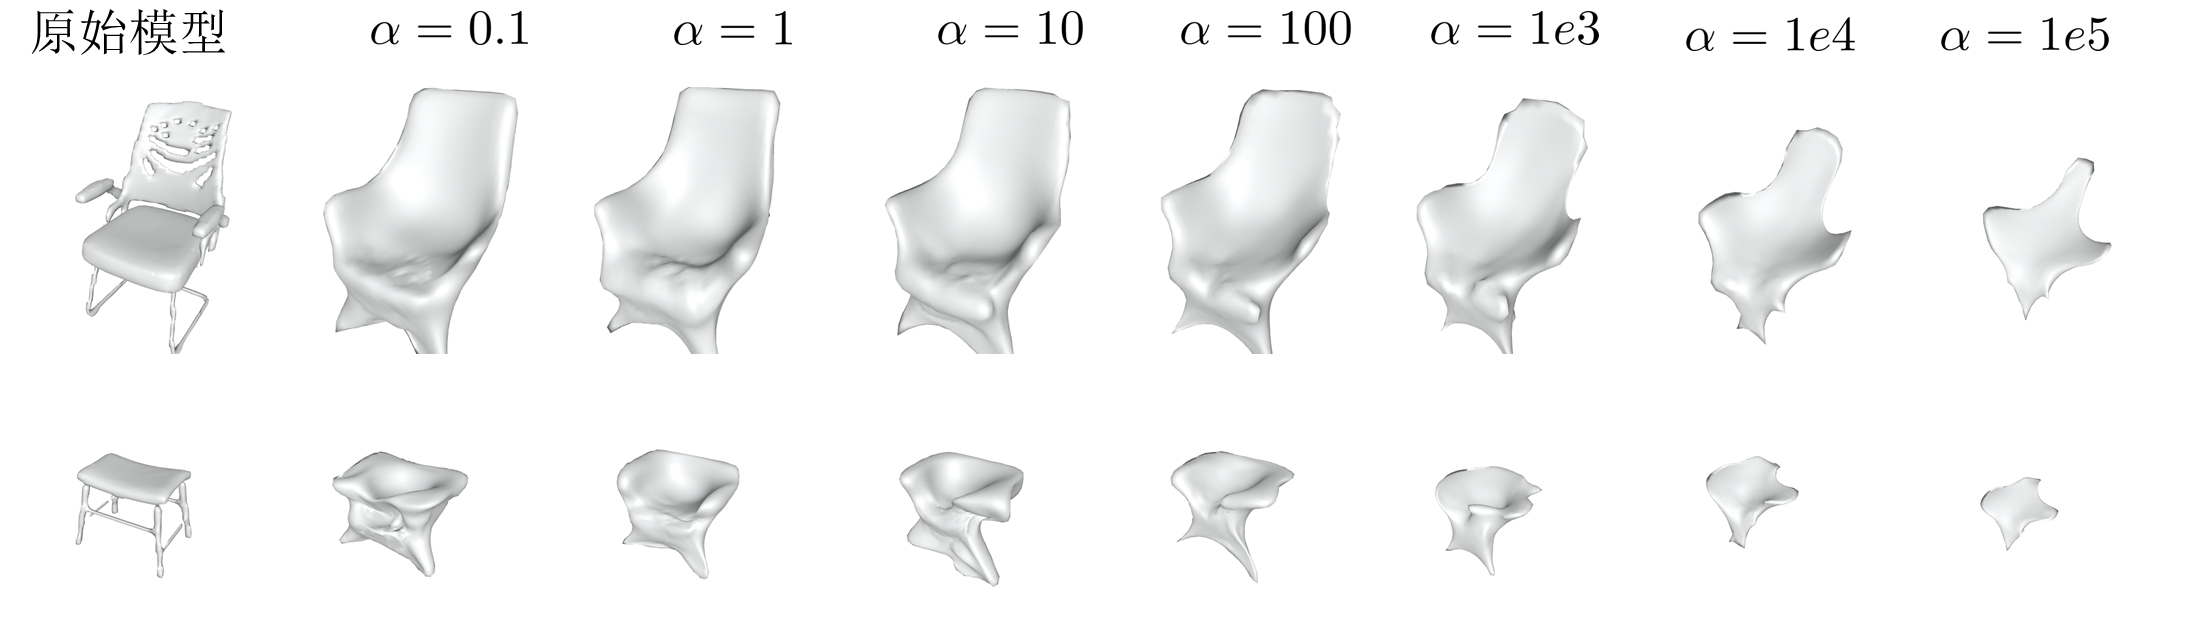
\includegraphics[width=0.9\linewidth]{Img/alpha_to_shape_2}
	\bicaption{损失$\mathcal{L}_{\text{inter}}$中的参数$\alpha$对归一化后的物体形状的影响。}{The effectiveness of $\alpha$ on the normalized shapes of the object.}
	\label{fig:alpha_shape}
\end{figure}

\subsection{定性分析}
% 在图\ref{fig:alpha_shape}中,展示了$\alpha$取不同值后,映射后的物体的形状变化,可以发现当$\alpha$取值太小,不利于物体形状映射学习到合适形状映射,因而导致了表\ref{tab:alpha_on_chairs}中所展示的重建精度的下降。

% \begin{figure}[!htbp]
% 	\centering
% 	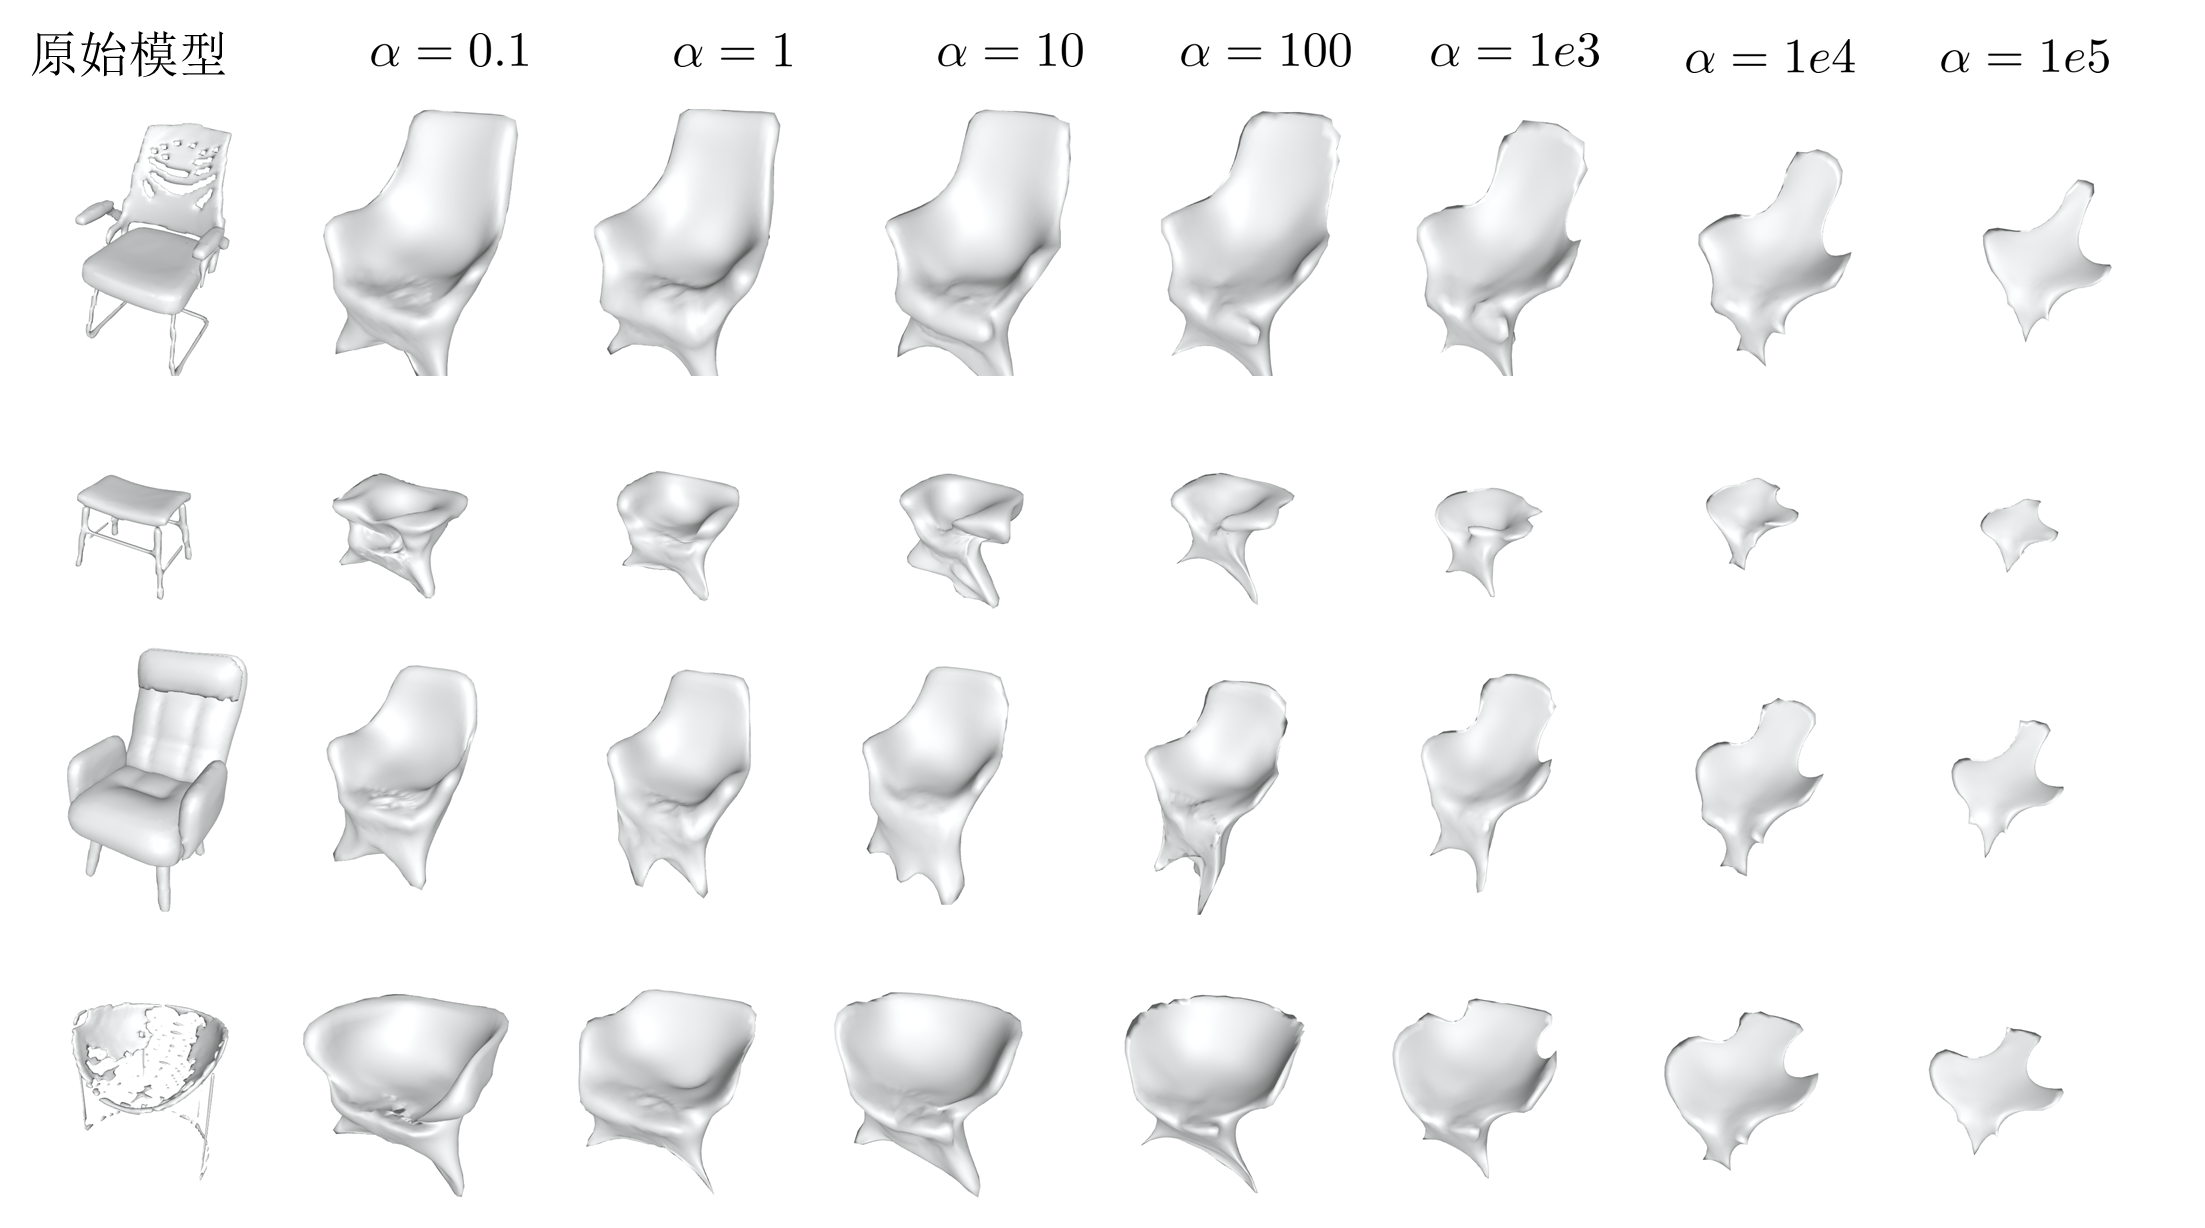
\includegraphics{Img/alpha_to_shape}
% 	\bicaption{损失$\mathcal{L}_{\text{inter}}$中的参数$\alpha$对归一化后的物体形状的影响。}{The effectiveness of $\alpha$ on the normalized shapes of the object.}
% 	\label{fig:alpha_shape}
% \end{figure}

在图\ref{fig:interaction_transfer}中对比了不同方法在不同物体上的迁移能力,给定参考的人-物交互实例,图中RT-based的方法将物体相对于人体的6D位姿迁移到不同的物体中,而offset-based方法将人和归一化后的物体之间的偏移量迁移到不同的物体中。从图中可以看出,如果只迁移物体的6D位姿,由于物体的形状有差异,从而导致在迁移过程中出现穿模和漂浮的现象,而基于偏移量的方法利用归一化后的物体形状,将偏移量在不同物体迁移,从而能够自适应对不同物体的位姿做调整。

\begin{figure}[!htbp]
	\centering
	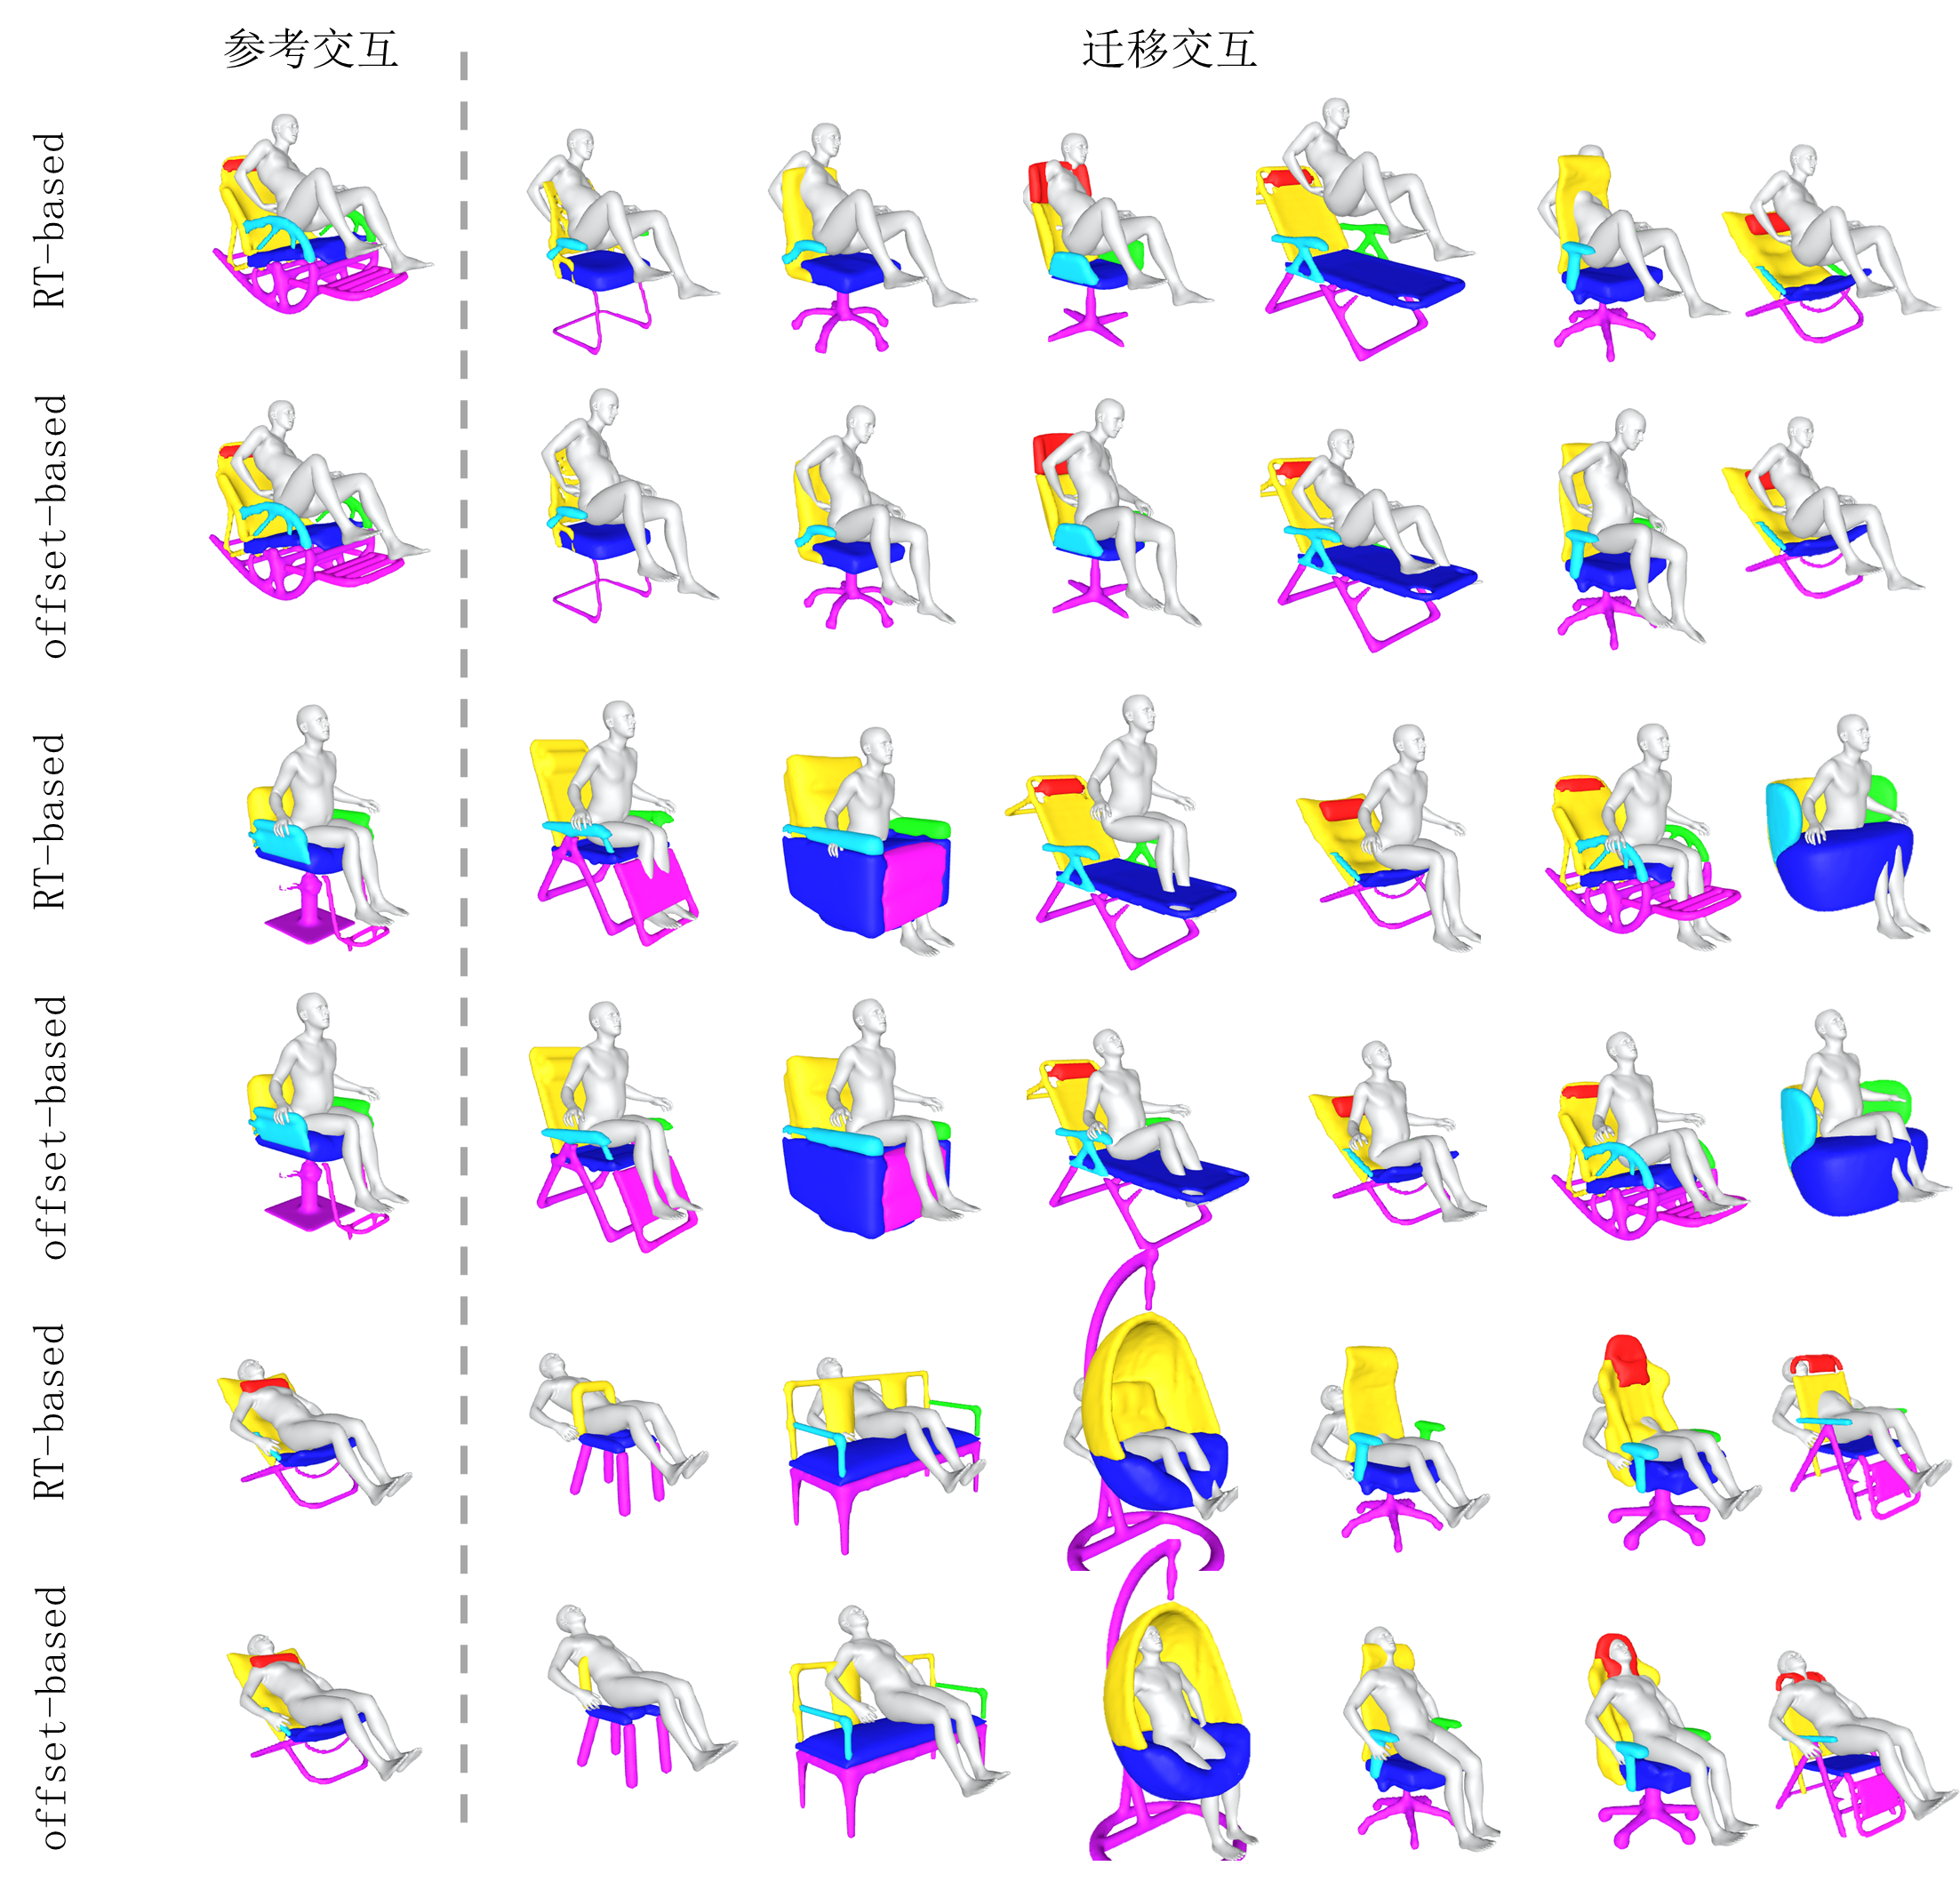
\includegraphics{Img/interaction_transfer_2}
	\bicaption{不同方法对交互关系在不同物体上的迁移能力对比。}{The comparison of the transfer ability to novel objects of different methods.}
	\label{fig:interaction_transfer}
\end{figure}

\section{本章小结}
本章提出使用物体形状的归一化函数将物体形状映射到统一形状空间中,并在该空间中,建立人和物体之间空间交互的编码。该空间关系的编码伴随物体形状映射函数的学习而动态调整,在训练该归一化映射函数时,使用到三个损失,第一个损失是人和物体之间偏移量损失,该损失使物体形状能够保持被映射后的物体形状仍然具有可交互性;第二个损失是平滑损失,该损失使物体模型表面保持平滑;第三类损失是增量PCA中投影矩阵的核范数,通过最小核范数来约束增量PCA所构建的隐式空间,从而增强相应物体形状的表示学习。通过在CHAIRS数据集实验验证,和基于RT的方法相比,该空间关系编码可以有效提高模型在新形状的物体上的泛化能力和迁移能力。